\begin{figure}
    \begin{center}
    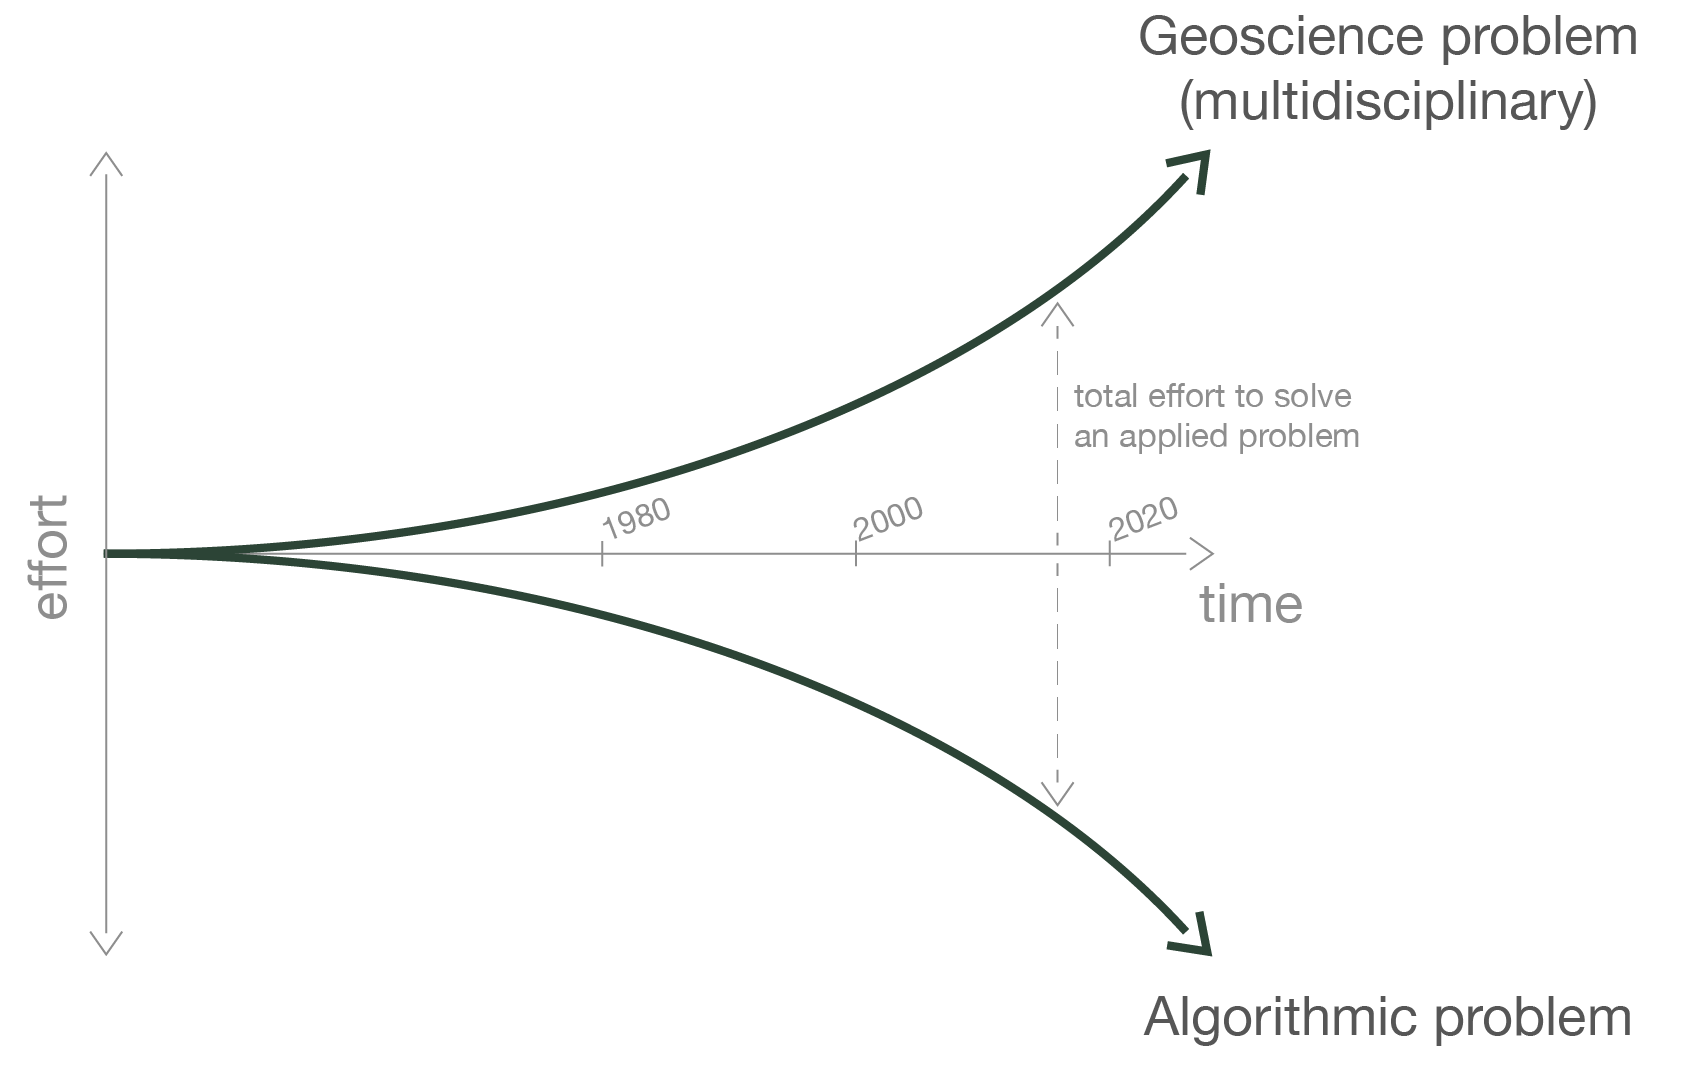
\includegraphics[width=0.8\columnwidth]{figures/diverging-curves-08.png}
    \end{center}
\caption{
    The plight of a researcher in geoscience. The horizontal axis reflects time, and the vertical distance away from this axis reflects the effort that a researcher must invest in order to solve a problem. The lower curve represents the effort required to solve an algorithmic problem and the upper curve represents the effort required to solve an integrated multi-disciplinary geoscience problem using algorithms. The distance between these two curves represents the total effort required to solve a state-of-the-art applied geoscience problem.
}
\label{fig:diverging-curves}
\end{figure}
